\chapter{Detectors\label{chap:calib}}

\section{Overview}



\section{Calibration}

\subsection{Collecting calibration spectra}

Any source with spectral lines in the energy range of interest can be
used for calibration. At the time of this writing, we are calibrating
all detectors with three sealed sources: $^{55}$Fe, which has spectral
lines at 5.9 and 6.5 keV; $^{57}$Co, with a line at 14.4 keV; and
$^{137}$Cs, which has a line at 32.2 keV.

For calibration, a long spectrum (at least 10 minutes) will be
acquired with every source following the steps below.
\begin{enumerate}
\item Start up the software and adjust the detector gain so that all
  peaks from the sources you are using will be within the detector's
  energy range.
\item \label{itm:affix} Using tape, affix one of the sources to the
  mylar on the end of the Cu pipe near the detector. Using the knobs
  on the stages, move the detector so that the Be window is close to
  the source.
\item In the software, acquire a short spectrum (30 seconds to 1
  minute) to ensure that the source peaks are visible and the detector
  dead time is not too high (should be <5\%). If necessary, move the
  detector and take another short spectrum.
\item \label{itm:acquire} Acquire a spectrum for at least 10 minutes,
  and then save it. You should use a large number of channels to get
  the best possible resolution---8192 is best.
\item \label{itm:reacquire} If the peaks in this 10 minute spectrum
  are still not very well resolved, take another spectrum for 10
  minutes or more. All spectra from a given sample can be added
  together for better statistics during the analysis.
\item After saving the spectrum from the previous source, remove the
  source and repeat steps \ref{itm:affix}-\ref{itm:reacquire} with a new
  source. Make sure to use the same gain and the same number of
  channels for each source. The acquisition time can vary from source
  to source. Repeat with all sealed sources.
\item When finished with the sealed sources, put them away in the lead
  source holder and place the holder in a locked cabinet.
\end{enumerate}
  
\subsection{Calibration data analysis}

%outline calib script
The script \path{blcontrol/scripts/calib.py} assists with the detector
calibration by fitting the peaks in each source spectrum, and then
fitting each of these peaks to a line which defines the detector
calibration parameters. The energy as a funciton of channel number,
$E(C)$, is found by fitting the source peak channels to a function of
the form
\begin{equation}
  \label{eq:calib-lin}
  E(C) = \frac{ C }{ \alpha \times G \times N } + E_0 \,
\end{equation}
where $G$ is the hardware gain and $N$ is the total number of channels. $\alpha$
and $E_0$, called the calibration factor and the offset, respectively, are
fitting parameters. Figures~\ref{fig:co57} and \ref{fig:linfit} show examples of
the plots output by the calibration script. The script will also print the
calculated values of the calibration factor and offset. You should inspect the
outputs to ensure that the values printed are sensible. Then,to enable the
calibration, paste these values into the appropriate location in
\texttt{blconf.txt} for the detector that you are calibrating. 

\begin{figure}
  \centering
  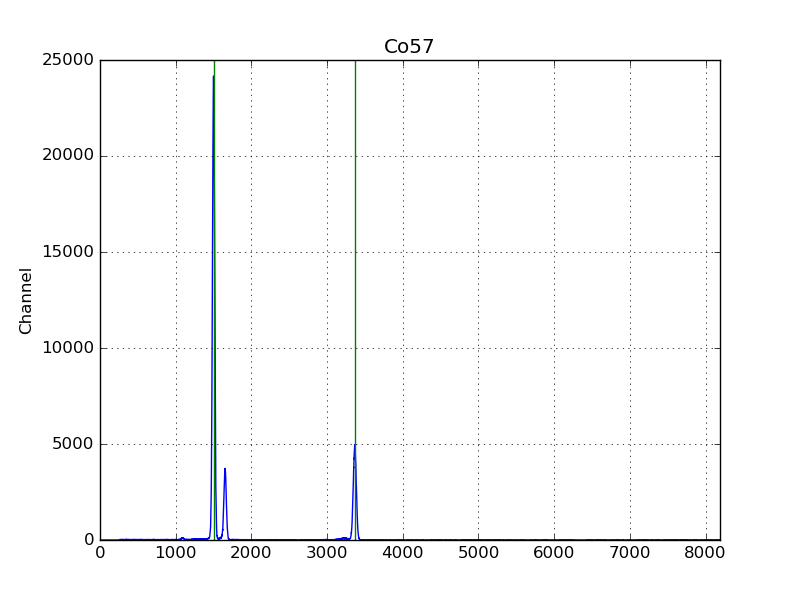
\includegraphics[width=0.7\textwidth]{Co57.png}
  \caption{\label{fig:co57} An example of a calibration spectrum from $^{57}$Co,
    with the peaks highlighted.}
\end{figure}

\begin{figure}
  \centering
  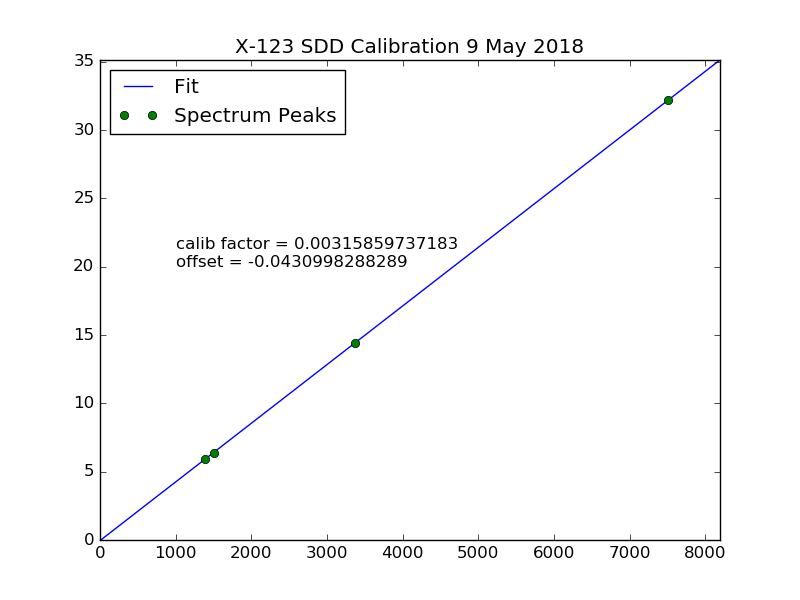
\includegraphics[width=0.7\textwidth]{linfit.png}
  \caption{\label{fig:linfit} This plot shows a linear fit to the peak channel
    as a function of energy for multiple calibration sources, calculated by the
    script \texttt{calib.py}. }
\end{figure}


%show example output plot

%%% Local Variables:
%%% mode: latex
%%% TeX-master: "Beamline_Manual"
%%% End:
